\chapter{Scripts}

This appendix chapter gives the scripts used in this notebook.

\section{\textit{Vim} Configuration \texttt{vimrc} Used in Section \ref{ch:tfe}}

\begin{lstlisting}
call plug#begin()
Plug 'vim-airline/vim-airline'
Plug 'joshdick/onedark.vim'
call plug#end()

inoremap jj <Esc>
noremap j h
noremap k j
noremap i k
noremap h i

noremap s <nop>
noremap S :w<CR>
noremap Q :q<CR>

syntax on
colorscheme onedark

set number
set cursorline
set wrap
set wildmenu

set hlsearch
exec "nohlsearch"
set incsearch
set ignorecase
noremap <Space> :nohlsearch<CR>
noremap - Nzz
noremap = nzz

noremap sj :set nosplitright<CR>:vsplit<CR>
noremap sl :set splitright<CR>:vsplit<CR>
noremap si :set nosplitbelow<CR>:split<CR>
noremap sk :set splitbelow<CR>:split<CR>
noremap <C-j> <C-w>h
noremap <C-l> <C-w>l
noremap <C-i> <C-w>k
noremap <C-k> <C-w>j
noremap J :vertical resize-2<CR>
noremap L :vertical resize+2<CR>
noremap I :res+2<CR>
noremap K :res-2<CR>

set scrolloff=3
noremap sc :set spell!<CR>
\end{lstlisting}

\chapter{Continuous Integration and Delivery}

This notebook is mainly about Linux. In this appendix chapter, the boundary of the notebook is slightly expanded to software development, which is quite often how Linux is used in practice.

Continuous integration and delivery (CI/CD) is both a philosophical concept and a bunch of technology that speeds up the development, testing and deployment cycle of a software. It has become a common and beneficial practice that collaborative projects that requires rapid update implement the practice.

This chapter introduces CI/CD as well as tools to carry out CI/CD. In particular, GitHub, a widely appreciated CI/CD integrated platform to manage and share collaborative projects, is briefly introduced. The introduction of later focuses on GitHub Action, the tool GitHub uses for CI/CD.

Some contents of this chapter come from \cite{honai2023cicd}.

\section{Agile VS Waterfall}

Agile and waterfall are both project management methodologies, one the counterpart of the other. Both of them are introduced here, starting with the more conventional waterfall model, then Agile.

\subsection{Waterfall}

Speaking of project proposal, development, testing and delivery cycle, it is fairly intuitive to following the following procedures:
\begin{enumerate}
	\item Understand requirements from the user.
	\item Design the architecture of the solution.
	\item Develop the solution.
	\item Test the solution.
	\item Deliver the solution and close the project.
	\item (Follow-up) maintenance of the solution.
\end{enumerate}
The kernel concept of waterfall, as its name indicates, is to ``follow the procedures and do not turn around''. When a previous step is considered completed, it is completed and should not be repeated. Otherwise, the flow would be interrupted. This is demonstrated by Fig. \ref{ch:cicd:fig:waterfall}.

\begin{figure}
	\centering
	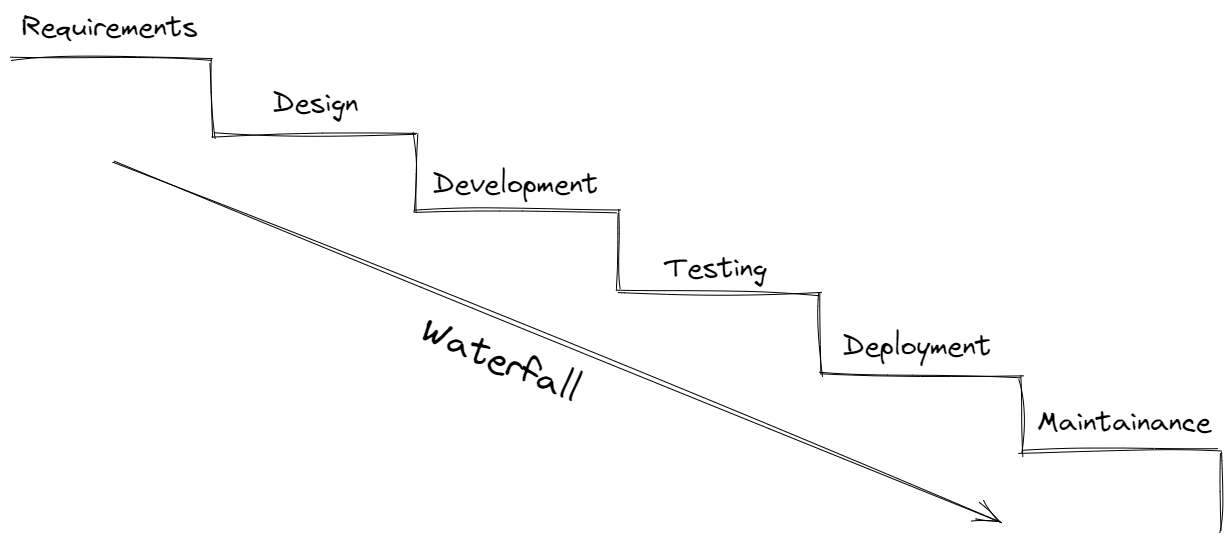
\includegraphics[width=300pt]{chapters/ap/figures/waterfall.png}
	\caption{Waterfall model.} \label{ch:cicd:fig:waterfall}
\end{figure}

With waterfall, a project can be designed, developed and deployed in a relatively efficient manner. However, there is one limitation: everything done in earlier steps is done and cannot be changed in later steps. This sets up a high bar on both the user and the developer. For example, in step 1 ``understand requirements from the user'', the user needs to illustrate all the requirements to the developer as they cannot be modified in later steps. Similarly, in step 2 ``design the architecture'', the developer needs to optimize the design to his best, as the architecture cannot be changed later.

Regrettably, with the rapid change in the market and the aggressive advent in technology today, it is challenging even for the smartest user and developer to determine all the requirements and designs in the beginning stage of the project. More likely, the requirements of the user have to change align with the market trend, and so does the design of the solution.

For a new feature to be added into the existing system, it is possible to simply start a new project flow for the new feature, and integrate it into the existing system later. However, integrating the new feature into the existing system can also be challenging when the design is complicated and coupled. The integration often introduces a blackout period of the system. If the system is already deployed, the customer experience would be affected by the blackout.

\subsection{Agile}

Agile is the counterpart of waterfall. It is proposed to tackle the aforementioned issue: rapid change of requirements and adaptations to new technology and tools. It allows continuous integration and deployment of new features into the system in a convenient and systematic way, without introducing blackout.

In agile architecture, each feature is separately modularized. Each feature, before deploying and integrating into production environment, circulates in its own “development and testing circle”, where it can be tested and reviewed iteratively by the developers and the customers, as shown below in Fig. \ref{ch:cicd:fig:agile}.

\begin{figure}
	\centering
	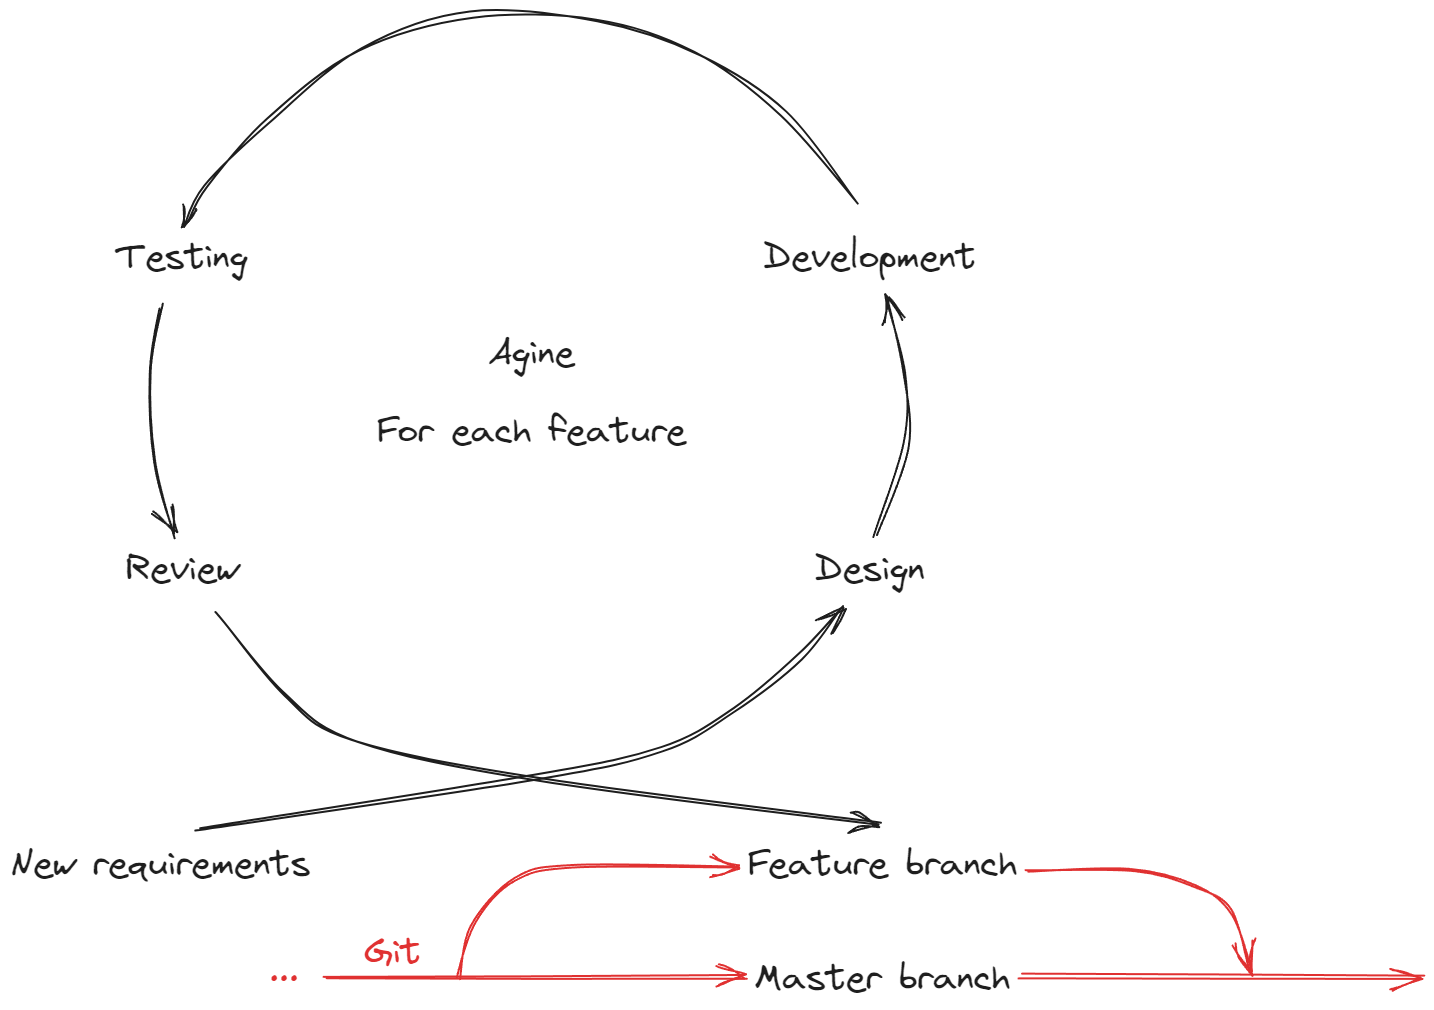
\includegraphics[width=300pt]{chapters/ap/figures/agile.png}
	\caption{Agile model.} \label{ch:cicd:fig:agile}
\end{figure}

Should there be any adjustment to the feature, just brings back the circle and improve the feature here, before releasing it to the production environment again.

Since modification becomes much easier in the agile development than in the waterfall development, agile development allows feedback collected during the development to be better reflected in the product. Whereas for waterfall development, the delivery is limited to the original design.

In parallel development where there are multiple features running in their associated circles, the developer can easily choose which feature branch and circles to prioritize. This gives the developer a clearer overview of what is happening and how to best answer to the customers immediate requirements.

\subsection{Roles in Agile-based Development}

On top of the agile development philosophy, roles and their responsibilities used in the development are defined. These roles may differ depending on the project management conventions in the team. The most commonly seen approach, namely \textbf{scrum}, is introduced in Table. \ref{ch:cicd:tab:agilerole}. 
\begin{table}[htbp]
	\centering
	\caption{Roles in Agile model.} \label{ch:cicd:tab:agilerole}
	\begin{tabularx}{\textwidth}{lX}
		\hline
		Role & Description \\
		\hline
		Product owner & Manage the entire program. He understands all the user requirements and progression of all features. He also signs off each feature when they are deployed. \\ \hdashline
		Scrum master & Lead the developer team as team manager or chief developer. \\ \hdashline
		Developer & Based on requirements, program the features. \\ \hdashline
		Tester & Design test cases to verify the efficacy of the developed feature. \\ \hdashline
		Operator/Supporter & Maintain the software \\
		\hline
	\end{tabularx}
\end{table}

In this role assignment, the product owner and scrum master come up with the product backlog, which clarify the sprints (tasks) and their priorities. The team then know which sprint they shall work on first.

In the case where the features are for a professional domain (such as economics, medical, etc.) that the developers cannot understand, business analysts are involved, who explains user requirements, design solution architecture, and setup test cases for the features.

For each sprint, sprint planning and sprint backlog are proposed that describes the schedule of the sprint. The team works on the sprint and host daily scrum meetings until the sprint is solved. Upon finishing of a sprint, sprint review is hosted that reviews and summarizes how the task is done.

\section{Continuous Integration Continuous Delivery (CI/CD)}

As the basics, pipeline is introduced. Pipeline is an important concept used in CI/CD. Consecutively CI/CD is introduced. 

\subsection{Pipeline}

Pipeline is a set of data processing elements connected in series, where the output of the upper stream processing is the input of the down stream processing. An example is shown in Fig. \ref{ch:cicd:fig:pipeline}.

\begin{figure}
	\centering
	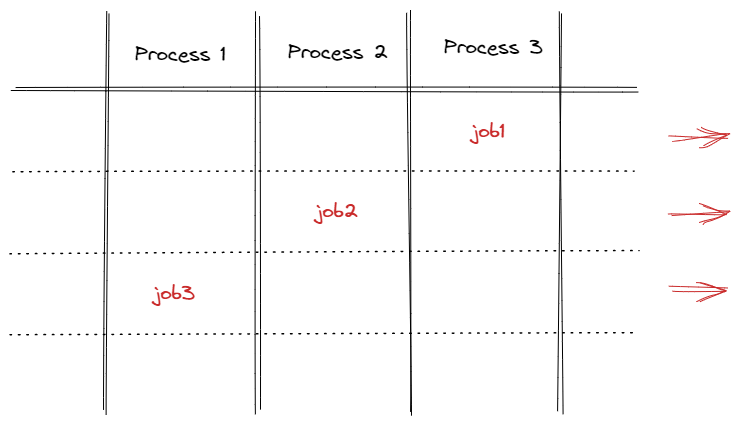
\includegraphics[width=300pt]{chapters/ap/figures/pipeline.png}
	\caption{Pipeline.} \label{ch:cicd:fig:pipeline}
\end{figure}

By using a pipeline and let multiple pipelines at different execution phase run in parallel, the efficiency of the system is increased.

The concept of pipeline is used in both CI and CD.

\subsection{Continuous Integration (CI)}

In the development of a sprint, new codes are rapidly developed, and they are rapidly compiled, packaged and tested. 

Conventionally, the integration of a new feature requires involvement from multiple parties. An example is given in Fig. \ref{ch:cicd:fig:conventionalintegration}. It includes the developer who program the software following users (or business analysts) requests, the integration team who integrates the new feature with the existing system and compile the code into packages, and the operations team who upload the new system into the pre-prod environment for real data testing, and the testers who audit the output of the program running in the pre-prod environment. 

Should there be any error along the way, the code is roll back the developer team for trouble shooting. When the new system with the updated code survives pre-prod environment, it is then pushed to the production environment.

\begin{figure}
	\centering
	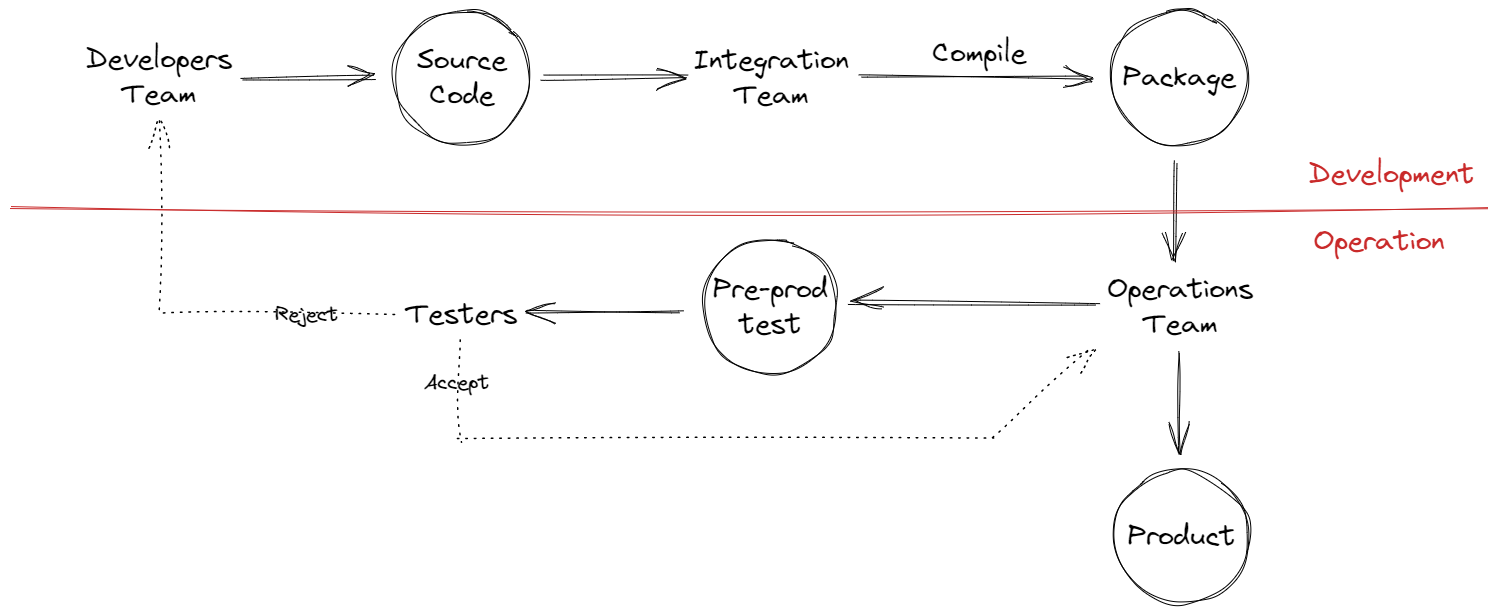
\includegraphics[width=350pt]{chapters/ap/figures/conventionalintegration.png}
	\caption{Conventional integration of new features.} \label{ch:cicd:fig:conventionalintegration}
\end{figure}

In practice, each cycle in Fig. \ref{ch:cicd:fig:conventionalintegration} can take a few days or even weeks as so many teams have to cooperate to make it happen. The latency mainly comes from
\begin{itemize}
	\item It takes time for the integration team to integrate different branches in the source code together, making sure that components from different branches function properly.
	\item When there is a defect, the flaws can be spotted only in the last stage of the iteration, i.e., testing.
\end{itemize}
This practically disallows very frequent update of the system in response to the rapid changes in requirements.

CI (together with CD which is introduced in later section) tries to solve the above problems. CI automates the ``development'' portion in Fig. \ref{ch:cicd:fig:conventionalintegration}, while CD automates the ``operation'' portion.

To speed up the development of new features, CI mainly adopts the following methods.
\begin{itemize}
	\item Use \textit{Git} to manage features. This simplifies the procedure of managing multiple under-development features and integrating them together. Integration is now managed by \textit{Git} following developers' intention.
	\item Use a build server to automatically compile the code into ready-for-delivery packages. The scrum master and senior developers can access the server and monitor the progression. Should there be a compiling error, the developer is notified immediately.
	\item The code, after compiling, is immediately tested in the build server using pre-defined test cases. If the code fails the test cases, the developer is immediately notified.
\end{itemize}

CI effectively removed ``integration team'' from the picture. The integration related tasks are split into small pieces and processed by automation tools, feature integration by \textit{Git}, and compiling by build server. During CI, the developer not only generates the codes, but also supervises \textit{Git} and build server. Should there be any error, the developer is notified immediately by the automation tools.

CI speeds up the developing cycle, from the receiver receiving requests from the user, to the point they have new system in the package ready for pre-prod testing.

\subsection{Continuous Delivery}

The package received from the development side contains the latest version of the system where a new feature is integrated. It is, however, not certain at this point whether the new feature works properly and how the system would behave as a whole with this new feature.

The sophisticated testing and deployment of the software features are done by the operations team.

Conventionally, operations team and the testers receive the updated package together with an instruction from the developers team. The instruction describes how the package shall be installed, and what test cases to use for auditing.

The operations team and the testers need to understand the instructions, and configure the pre-prod environment accordingly for the testing. The testers then uses varieties of scenarios to test the performance of the software. Bugs, if any, are reported to the developers team. If no bugs are spotted, the testers notify the operation team to release the package into production environment.

Some drawbacks of the above procedures are:
\begin{itemize}
	\item The developers team needs to give detailed and precise instruction to the operations team, and the developers may make mistakes or missing something in the instruction, especially regarding environment configuration.
	\item Too many human interactions, which slow down the process and generates human error. The entire procedure usually take about a whole day.
\end{itemize}

Continuous delivery is a software development practice that allows software to be released to production at any time. The key philosophy is that, under CI infrastructure, the code should be always ready to be released.

Firstly, form the instruction file using computer languages, so that the configuration of environments and installation of packages can be done automatically. Technologies such as containerizations can help with this procedure.

Secondly, all the test scripts shall be pre-programmed, so that they can be executed automatically. If no bugs are detected in the test, the package is to be released automatically.

Both instruction files for environment setup, package installation, and testing plan, can all be stored and managed in the repository together with the source code. The operation team can now join the developers team. They are essentially all working on codes, just with some differences in the focusing areas.

The above procedures form the release pipeline, and it makes it technically possible to release a package to production environment at any time. In practice, there is often still the quality insurance team that sign off the packages before the release, just in case.


\section{GitHub Action}





















